% This is a LaTeX document for a CV/Resume
\documentclass[10pt,a4paper]{article}
\usepackage[utf8]{inputenc}
\usepackage[T1]{fontenc}
\usepackage{geometry}
\geometry{margin=1in}
\usepackage{graphicx}
\usepackage{parskip}
\usepackage{titlesec}
\usepackage{color}
\usepackage{xcolor}
\usepackage{enumitem}
\usepackage{hyperref}
\usepackage{fontawesome5}

\titleformat{\section}{\large\bfseries\uppercase}{\thesection}{1em}{}
\titleformat{\subsection}[runin]{\bfseries}{\thesubsection}{0.5em}{}[.]

\pagestyle{empty}
\hypersetup{
    colorlinks=true,
    linkcolor=blue,
    urlcolor=blue
}

\begin{document}

% Header with image
\begin{minipage}[t]{0.7\textwidth}
    \textbf{\LARGE Ryan Matthews}\\
    \vspace{0.1cm}
    \href{mailto:ryanjmatthews@gmail.com}{ryanjmatthews@gmail.com} \quad
    \href{https://linkedin.com/in/ryan-j-matthews}{LinkedIn} \quad
    \href{https://github.com/Darainer}{GitHub} \quad
    +49 176 34599887\\
    \vspace{0.3cm}
    Engineering leader with over 10 years of experience in automated driving development, delivering business outcomes in both technical and product leadership roles. Passionate about building commercially successful software and AI rich products.
\end{minipage}
\hfill
\begin{minipage}[t]{0.25\textwidth}
    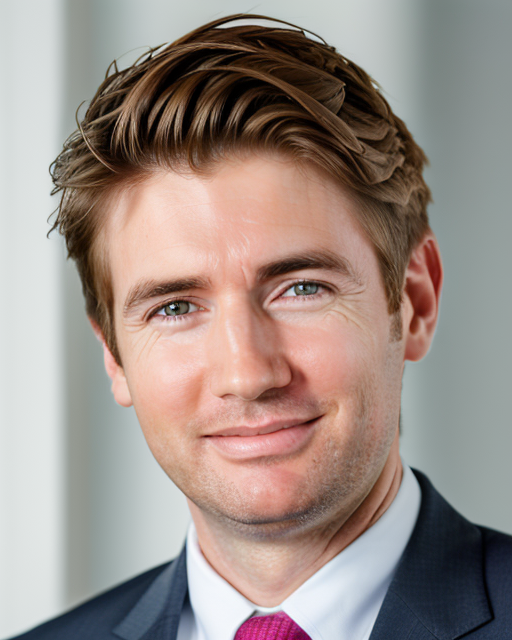
\includegraphics[width=\linewidth]{profile_pic_ryan.png}
\end{minipage}

\vspace{0.5cm}

\section*{Work Experience}

\textbf{SYSTEM ARCHITECT ADAS/AD}, Luminar, Munich \hfill \textit{Jul 2022 – Present}\\
\begin{itemize}[leftmargin=*]
    \item Provide technical direction for the product portfolio, encompassing Software, SoC, and Lidar.
    \item Successfully drove structural changes in software product strategy by analyzing shifts in customer sourcing trends, influenced by the adoption of novel deep learning architectures.
    \item Designed and socialized a software toolchain to support multidisciplinary development.
\end{itemize}

\textbf{PRODUCT OWNER ACTIVE SAFETY}, Luminar, Munich \hfill \textit{Sep 2020 – Jun 2022}\\
\begin{itemize}[leftmargin=*]
    \item Led the greenfield development of a lidar-only, NCAP 2023 compliant active safety software stack and successfully demonstrated at \href{https://ces.tech}{CES 2022} and further innovations in \href{https://ces.tech}{CES 2023}.
    \item Outlined, aligned and executed on product vision to push state of the art in active safety.
    \item Built a high performing ADAS team from a group of developers without domain knowledge.
\end{itemize}

\textbf{PRODUCT OWNER ADAS}, Samsung Electronics, Munich \hfill \textit{Apr 2019 – Sep 2020}\\
\begin{itemize}[leftmargin=*]
    \item Led the camera-only AEB NCAP 2022+ product development for Samsung SoC based solution.
    \item Technical direction for algorithm development on the full end to end software chain.
\end{itemize}

\textbf{SENIOR DEVELOPER}, Zenuity (JV Volvo / Autoliv), Munich \hfill \textit{Mar 2018 – Mar 2019}\\
\begin{itemize}[leftmargin=*]
    \item Led the successful migration of the existing codebase into a modern CI/CD environment and the transition to data driven feature development.
    \item Delivered on key business outcome to have daily KPI evaluation on the data lake.
    \item Provided local mentoring for ADAS function and algorithm development.
\end{itemize}

\textbf{LEAD FEATURE DEVELOPER}, Autoliv Electronics, Munich \hfill \textit{Oct 2016 – Mar 2018}\\
\begin{itemize}[leftmargin=*]
    \item Developed robust tracking and control algorithms for a novel camera-only ACC system.
    \item Successfully demonstrated system to OEM customers, resulting in program business wins.
\end{itemize}

\textbf{ENGINEERING CONSULTANT}, TESIS DYNAware, Munich \hfill \textit{Feb 2011 – Sep 2016}\\
\begin{itemize}[leftmargin=*]
    \item Technical project management up to 10 team members and > \$1 million budget.
    \item Consistently successful in securing contract extensions and acquisition of new software customers.
    \item Developed vehicle functions and algorithms for ADAS + ESP applications (German OEMs/ Tier1s).
\end{itemize}

\textbf{MECHATRONIC ENGINEER}, Australian Submarine Corporation, Perth \hfill \textit{Jan 2007 – Apr 2010}\\
\begin{itemize}[leftmargin=*]
    \item Submarine control system design and in-service support on operational submarines.
\end{itemize}

\vspace{0.4cm}

\section*{Education}

\textbf{B.Eng (Hons), Mechatronic Engineering}, University of Adelaide\\
First Class Honours, Dean's List, Aerospace Project Award

\textbf{Bachelor of Economics}, University of Adelaide\\
Major in mathematical modelling and statistical analysis

\vspace{0.4cm}

\section*{Skills}
C++, Python, Model-Based Design, ISO 26262, AUTOSAR, Agile Product Ownership

\vspace{0.4cm}

\section*{Languages}
English (Native), German (Full Professional)

\end{document}